\documentclass{amsart}

\usepackage[english]{babel}
\usepackage[utf8]{inputenc}
\usepackage{graphicx}
\usepackage{mathtools}
\usepackage{amsthm}
\usepackage{amsfonts}
\usepackage{hyperref}
\usepackage[singlelinecheck=false]{caption}
\usepackage[backend=biber,url=true,doi=true,eprint=false,style=alphabetic]{biblatex}
\usepackage{enumitem}
\usepackage[justification=centering]{caption}
\usepackage{indentfirst}
\usepackage{algorithm}
\usepackage{algpseudocode}
\usepackage{listings}

\addbibresource{references.bib}

\makeatletter
\def\subsection{\@startsection{subsection}{3}%
  \z@{.5\linespacing\@plus.7\linespacing}{.1\linespacing}%
  {\normalfont\itshape}}
\makeatother

\DeclareMathOperator*{\argmin}{arg\,min}
\DeclareMathOperator*{\argmax}{arg\,max}

\newcommand\defeq{\mathrel{\overset{\makebox[0pt]{\mbox{\normalfont\tiny\sffamily def}}}{=}}}

\algrenewcommand\algorithmicrequire{\textbf{Input}}
\algrenewcommand\algorithmicensure{\textbf{Output}}

\captionsetup[table]{labelsep=space}

\theoremstyle{plain}

\newtheorem*{definition}{Definition}
\newtheorem{theorem}{Theorem}
\newtheorem{proposition}{Proposition}
\newtheorem{exercise}{Exercise}

\newenvironment{solution}{\begin{proof}[Solution]}{\end{proof}}

\newcommand{\set}[1]{\mathcal{#1}}
\newcommand{\pr}{\mathbb{P}}
\renewcommand{\implies}{\Rightarrow}

\setlength{\parskip}{1em}

\lstset{frameround=fttt,
  language=[5.3]Lua,
	numbers=left,
	breaklines=true,
	keywordstyle=\bfseries,
	basicstyle=\ttfamily,
}

\newcommand{\code}[1]{\lstinline[mathescape=true]{#1}}
\newcommand{\mcode}[1]{\lstinline[mathescape]!#1!}

\title[]{11. Constraint-based Structure Learning}
\author[]{Renato Lui Geh\\NUSP\@: 8536030}

\begin{document}

\begin{abstract}
  This document contains the solutions to the proposed exercises from Lecture 11.
  \vspace*{-2.5em}
\end{abstract}

\maketitle

\section{Solutions}

\begin{exercise}
  Learn a PDAG using d-separation as oracle in each of the following structures.
\end{exercise}

\begin{solution}
  For the first structure let's consider the following sentences
  \begin{align*}
    &B\perp C | A\\
    &A\perp D | B
  \end{align*}
  We know these two to be true from our oracle. Therefore we can remove edges $A-D$ and $B-C$
  with witness sets $\set{Z}_{AD}=\{B\}$ and $\set{Z}_{BC}=\{A\}$ respectively. These two sentences
  are the only relevant (in)dependencies for this first step. Now we must find convergent
  connections. Our oracle shows that we only have one convergent connection, since
  \begin{equation*}
    B\not\perp C | D
  \end{equation*}
  From there we have the following resulting PDAG\@:
  \begin{figure}[h]
    \centering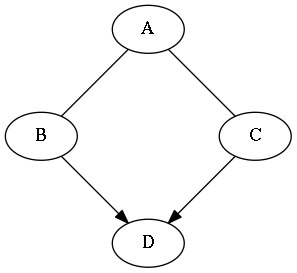
\includegraphics[scale=0.3]{graphs/ex1_a.png}
  \end{figure}
  Edges $A-B$ and $A-C$ are both undirected since $B-A-C$ can either be a serial or divergent
  connection, but it cannot be convergent.

  For the second structure we have the following independencies
  \begin{align*}
    &A\perp D|C\\
    &B\perp C|\emptyset
  \end{align*}
  We then remove edges $A-D$ with $\set{Z}_{AD}=\{C\}$ and $\set{Z}_{BC}=\emptyset$. The next step
  is to find potential immoralities (convergent connections). From the definition of convergent
  connections we can then ask the oracle
  \begin{equation}
    \text{Given connection $B-A-C$,~} A\in \set{Z}_{BC}?\label{ex1-b-1}
  \end{equation}
  \begin{equation}
    \text{Given connection $B-D-C$,~} D\in \set{Z}_{BC}?\label{ex1-b-2}
  \end{equation}
  Who is going to return false to both these questions. We now know that $B\to A\gets C$
  from~\ref{ex1-b-1} and $B\to D\gets C$ from~\ref{ex1-b-2}. This gives the following final PDAG\@:
  \begin{figure}[h]
    \centering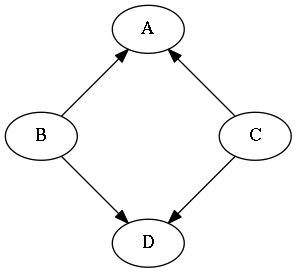
\includegraphics[scale=0.3]{graphs/ex1_b.png}
  \end{figure}

  For the last structure:
  \begin{align*}
    &A\perp D|B\\
    &D\perp A|C\\
  \end{align*}
  This removes edges $A-D$ with $\set{Z}_{AD}=\{B,C\}$. Testing immoralities, we have that:
  \begin{align*}
    &B\not\perp C|D \implies B\to D\gets C\\
    &A\not\perp B|C \implies A\to C\gets B\\
  \end{align*}
  This gives the final PDAG
  \begin{figure}[h]
    \centering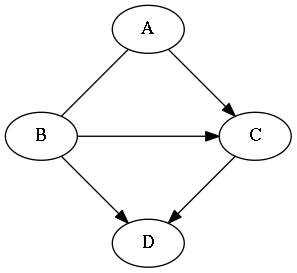
\includegraphics[scale=0.3]{graphs/ex1_c.png}
  \end{figure}
  The undirected edge $A-B$ tells us that there are equivalent networks with $A\to B$ and
  $A\gets B$ that do not contradict the independencies we assumed.
\end{solution}

\begin{exercise}
  Answer the following questions:
  \begin{enumerate}[label=(\roman*)]
    \item Give an example where the PC algorithm reconstructs the wrong structure due to the
      presence of a single wrong answer of the oracle.
    \item Give an example where the algorithm reconstructs the correct skeleton but makes a single
      mistake when extracting the immoralities (and hence learns the wrong structure).
  \end{enumerate}
\end{exercise}

\begin{solution}~\\

  \textit{(i)} Consider the solution to the second structure of Exercise 1. Had our oracle answered
  the query $A\perp D|C$ as false, we wouldn't have removed the edge $A-D$, which would've caused
  the resulting PDAG to be different then what we found.

  \begin{figure}[h]
    \centering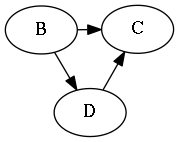
\includegraphics[scale=0.45]{graphs/ex2.png}
    \caption{}\label{ex2}
  \end{figure}


  \textit{(ii)} Take the solution to the third structure of Exercise 1 as example. If the query
  $B\perp C|D$ had returned true, we then wouldn't have had a convergent connection $B\to D
  \gets C$. Instead, because of the Acyclicity step of the PC algorithm, we would've had a
  a different $BCD$ connection, as shown in Figure~\ref{ex2}.
\end{solution}

\newpage

\printbibliography[]

\end{document}
